\documentclass[border=10pt]{standalone}
\usepackage{tikz}
\begin{document}
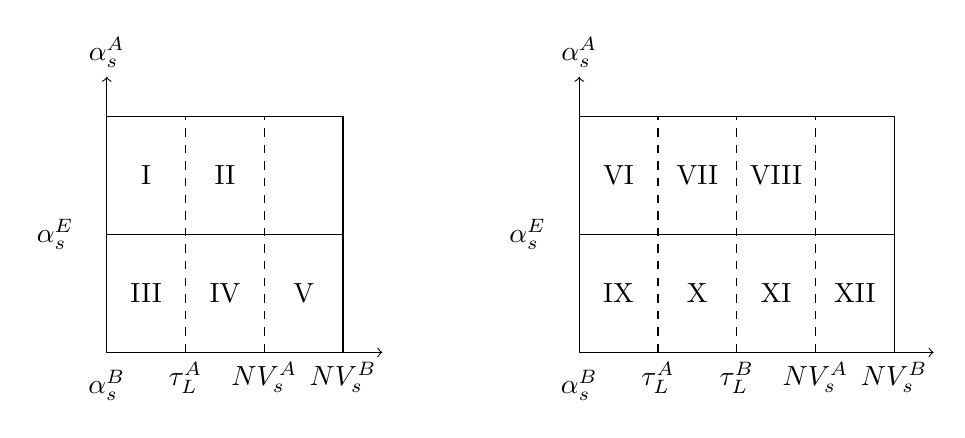
\begin{tikzpicture}
% Left diagram
\draw (0,0) rectangle (3,3);
\draw (0,1.5) -- (3,1.5);
\draw[dashed] (1,0) -- (1,3);
\draw[dashed] (2,0) -- (2,3);
\draw[->] (0,0) -- (3.5,0);
\draw[->] (0,0) -- (0,3.5);
\node[above] at (0,3.5) {$\alpha^A_s$};
\node[below] at (0,-0.1) {$\alpha^B_s$};
\node[left] at (-0.3,1.5) {$\alpha^E_s$};
\node[below] at (1,0) {$\tau^A_L$};
\node[below] at (2,0) {$NV^A_s$};
\node[below] at (3,0) {$NV^B_s$};
\node at (0.5,2.25) {I};
\node at (1.5,2.25) {II};
\node at (0.5,0.75) {III};
\node at (1.5,0.75) {IV};
\node at (2.5,0.75) {V};

% Right diagram
\begin{scope}[xshift=6cm]
\draw (0,0) rectangle (4,3);
\draw (0,1.5) -- (4,1.5);
\draw[dashed] (1,0) -- (1,3);
\draw[dashed] (2,0) -- (2,3);
\draw[dashed] (3,0) -- (3,3);
\draw[->] (0,0) -- (4.5,0);
\draw[->] (0,0) -- (0,3.5);
\node[above] at (0,3.5) {$\alpha^A_s$};
\node[below] at (0,-0.1) {$\alpha^B_s$};
\node[left] at (-0.3,1.5) {$\alpha^E_s$};
\node[below] at (1,0) {$\tau^A_L$};
\node[below] at (2,0) {$\tau^B_L$};
\node[below] at (3,0) {$NV^A_s$};
\node[below] at (4,0) {$NV^B_s$};
\node at (0.5,2.25) {VI};
\node at (1.5,2.25) {VII};
\node at (2.5,2.25) {VIII};
\node at (0.5,0.75) {IX};
\node at (1.5,0.75) {X};
\node at (2.5,0.75) {XI};
\node at (3.5,0.75) {XII};
\end{scope}
\end{tikzpicture}
\end{document}